%%%%%%%%%%%%%%%%%%%%%%% file typeinst.tex %%%%%%%%%%%%%%%%%%%%%%%%%
%5
% This is the LaTeX source for the instructions to authors using
% the LaTeX document class 'llncs.cls' for contributions to
% the Lecture Notes in Computer Sciences series.
% http://www.springer.com/lncs       Springer Heidelberg 2006/05/04
%
% It may be used as a template for your own input - copy it
% to a new file with a new name and use it as the basis
% for your article.
%
% NB: the document class 'llncs' has its own and detailed documentation, see
% ftp://ftp.springer.de/data/pubftp/pub/tex/latex/llncs/latex2e/llncsdoc.pdf
%
%%%%%%%%%%%%%%%%%%%%%%%%%%%%%%%%%%%%%%%%%%%%%%%%%%%%%%%%%%%%%%%%%%%


\documentclass[runningheads,a4paper]{llncs}

\usepackage[latin1]{inputenc}
\usepackage{graphicx,color,url}
\usepackage[dvips]{epsfig}
\usepackage{verbatim}
\usepackage{tikz}
\usepackage{subfigure}

\usetikzlibrary{shapes,arrows}
\usetikzlibrary{calc,patterns,snakes,decorations.pathmorphing,decorations.markings}
\usetikzlibrary{positioning}

\providecommand{\tabularnewline}{\\}

\usepackage{amssymb}
\setcounter{tocdepth}{3}
\usepackage{graphicx}

\usepackage{url}
\urldef{\mailsa}\path|salemohammed@gmail.com|
\urldef{\mailsb}\path|amorag@geneura.ugr.es, jjmerelo@gmail.com|
%\urldef{\mailsc}\path| fergunet@gmail.com|
\newcommand{\keywords}[1]{\par\addvspace\baselineskip
	\noindent\keywordname\enspace\ignorespaces#1}

\begin{document}
	
\mainmatter  % start of an individual contribution
	
	% first the title is needed
\title{Evolving a TORCS Fuzzy driver using Genetic Algorithms}
	
	
	%\titlerunning{Driving in TORCS using modular fuzzy controllers}
	
	
	
	
%	\author{Mohammed Salem* \inst{1} \and Antonio Miguel Mora \inst{2}\and Juan Julian Merelo \inst{2} \and Pablo Garc\'ia-S\'anchez \inst{3}}
% Antonio - The submission is blind. ;)
\author{First Author \inst{1} \and Second Author \inst{2} and Third Author \inst{3}}	
	
	%\authorrunning{M. Salem et al}
	% (feature abused for this document to repeat the title also on left hand pages)
	
	% the affiliations are given next; don't give your e-mail address
	% unless you accept that it will be published
%	\institute{University of Mascara, Algeria\\
%		\mailsa\\
%		Department of Architecture and Computer Technology
%		University of Granada, Spain\\
%		\mailsb\\
%		Universiy of C\'adiz, Spain
%		\\
%		\mailsc\\
%	}
% Antonio - The submission is blind. ;)

\institute{First Institute
  \and
  Second Institute
  \and
  Third Institute}
% Still need to get the space right - JJ
	%
	% NB: a more complex sample for affiliations and the mapping to the
	% corresponding authors can be found in the file "llncs.dem"
	% (search for the string "\mainmatter" where a contribution starts).
	% "llncs.dem" accompanies the document class "llncs.cls".
	%
	
%	\toctitle{}
%	\tocauthor{}
	\maketitle
	\begin{abstract}
		
          This work presents an evolutionary approach to optimize the
          parameters of Fuzzy-based controller for an autonomous
          driver for the open simulated car racing game (TORCS). Using
          evolution, we intend to improve a modular fuzzy agent
          designed to determine the optimal target speed and steering
          angle during the race. The challenge in this kind of fuzzy
          systems is the design of the membership functions, which is
          usually done through a trial and error process.
%          These kinds of controllers have a big drawback, which is their membership function parameters are tuned by a trial-error process.
In this paper, a real-coded Genetic Algorithm 
% Antonio - TODO: Extend the description of the algorithm.
has been applied to find the best values for these parameters,
obtaining a robust design for the TORCS controller.
The evolved drivers were compared %Pablo: compared with other controllers? Explain
and  evaluated in practice and
real races with integrated drivers of  TORCS, yielding very good results mainly in tracks that have
many turning points, which are, in turn, the most difficult for any
autonomous agent. %Is this true? If this is explained in next sections, do not forget to add a reference to validate it.
% Mohammed- The fuzzy controller in the previous paper is designed so to detect turns and break late makind a trade-off between safety and maximise the speed
% Antonio - TODO: describe the experiments performed and say something else about the results.
%%%

% What do you mean by "in practice *and* realistic races". - JJ

%Mohammed- Practice : alone race , real race : with opponents from TORCS
\end{abstract}

\keywords{Videogames, Fuzzy Controller, TORCS, Steering control, Optimization, Genetic Algorithms}

% Antonio - I have rewritten the abstract. It was very similar to the one of last year. ;)

%%%%%%%%%%%%%%%%%%%%%%%%%%%%%%%   INTRODUCTION   %%%%%%%%%%%%%%%%%%%%%%%%%%%%%%%
	%
\section{Introduction}
\label{sec:intro}

% Antonio: TODO - write the Introduction.
Autonomous driving is a very interesting research topic recently
supported by many vehicle manufacturers. The final aim is to create
real self-driving cars that can move in everyday roads and streets or, for
that matter, in a desert or hostile environment. This objective is
complemented with the reduction of fuel consumption and the
maximization of its efficient use, along with the car safety and the
driver comfort in some cases; all these improvemets with the implied
constraint that no accidents should take place.  

Optimization in car racing games can be situated in that context, with
solutions obtained there having utility beyond the game itself; this
explains the popularity of car racing games challenges, which are
usually performed using game simulators. The Open Racing Car Simulator
(TORCS) \cite{WebTORCS} is a realistic racing simulator with a
sophisticated engine used for many standalone racing competition
challenges every year. This fact, combined with the large gaming
community and the ability to compare controllers, have made TORCS the
most used simulator in the field of autonomous driving \cite{LFAG,Guadarrama2008,SAES2012,Floreano2004}. 
% Antonio - add some references about research in TORCS (from those commented in the State of the art)
% But don't leave that that way. Either you add them, or put the comment, but don't leave it that way - JJ
% Mohammed -done
% Great :-) - JJ
Many kinds of controllers have been used in this simulator, but one of the most efficient controllers so far are fuzzy-based ones, as they simulate in part the human
reasoning when driving \cite{CarRacing_Pelta09,PerezEvolvingFuzzy09,torcs2012}. % More references here - JJ %Mohammed- done
In this line, the authors presented previously
an approach in which two specialised fuzzy controllers were combined
to decide the car's steering angle and desired speed in every single
point during a race \cite{evo17_blind}.  
% Antonio - citation to our previous work without authors nor title since this is a blind revision process
% Antonio - Mohammed, was these factors computed every small amount of time or just in some parts of the track, such as in every curve?
% Mohammed - They are computed every race tick ( we have any previous knowledge about the track parts: straight or curves)

The obtained results were promising, but the performance of the autonomous driver showed some flaws in difficult tracks - where `external' factors affected the asphalt - and against the most competitive rivals. 
We argue here that the major disadvantage of this approach is that the parameters of the controllers' fuzzy membership functions were defined following a trial/error process in the absence of experts to do so.

Thus, in this work we consider the selection of the best values for these parameters as an optimization problem, so we have applied an evolutionary algorithm to obtain them. Concretely, we propose to apply a real-coded Genetic Algorithm (GA) \cite{realcodedGA1998} 
% Antonio - Look for a citation to a real-coded GA?
% Mohammed- Done
with this purpose. The considered approach requires - in addition to a good codification of solutions and selection of operators - the choice of an adequate cost function (fitness), due to the uncertainty and noisiness of the problem itself, so two different implementations have been studied.


The genetic-fuzzy  based controller is evaluated in practice race first and then in a real race against different drivers in TORCS.
Our results show that the proposed approach can successfully
evolve the fuzzy controller membership parameters giving good performances in terms of damage avoidance and race time, our results suggest that genetic algorithms with the selected fitness fitness  are well-suited for finding 
the best trade-off between the two objectives of any racing controller (Damage, Speed).
% Antonio - TODO: Comment about the obtained results
% Mohammed- Done
%%%%%%%%%%%%%%%%%%%%%%%%%%%%%%  STATE OF THE ART  %%%%%%%%%%%%%%%%%%%%%%%%%%%%%%
\section{State of the Art}
\label{sec:soa}

% Antonio: TODO - write the State of the art.
% Revise the state of the art so that it tells something, and is not only "this guy does this, while that guy does that". It has to establish the "state of the art", what is being done in the area so that we prove that it's an improvement. 

Evolutionary algorithms have been used by several researchers in
driving a racing car in TORCS simulator.
% Name the authors, don't simply say "authors of" - JJ
Loiacono et al \cite{AutogenEvo2011} have  applied a single-objective and a multi-objective
real-coded genetic algorithm to the automatic generation of tracks for high-end
racing games while  \cite{Montecarlo2016} proposes a new framework of applying Monte Carlo Tree Search to the simulated car racing by  building the search tree in a discretized game-state space and then determine the action from the selected target game state to avoid the need to discretize the action space. 

Another application of evolutionary algorithms was to determine the optimal trajectory of a lap in a known circuit \cite{drivingGA2008}  but their approach suffers from  problem that the obtained trajectory 
in the evolving process depends highly on the initial state of the car. In the same context, \cite{GaRaceLine2010} tried to design a novel approach to compute the racing line
without any human intervention using genetic algorithm to find the best trade-off between
the minimization of two conflicting objectives: the length and
the curvature of the racing line.

Floreano et al. \cite{Floreano2004}, used a GA for tuning up a neural network which visually
recognizes edges, corners and height, resembling strategies observed in simple
insects which obtained results that performed equal or better than well trained
human drivers tested on the same circuits. 
%%%%%%%%%%%%%%%%%%%%%%%%%%%%%%%%%%%%%%%%
% Make a statement about the "state of the art", like "in general, EAs
% have obtained good results with the constraint of the underlying
% controller that is being optimiize - JJ

% If you are introducing another topic, you have to relate with the
% previous paragraph - JJ
In \cite{SAES2012}, the authors design a competitive driving controller in TORCS  by optimizing the
parameters of an autonomous car controller using self adaptive
evolutionary strategies (SAESs) which co-evolve solutions and mutation steps for each parameter. %Pablo: how we can use this referene to validate ours? Which is our selling-point/differenciation?

% FUZZY + EAs
% Always "narrate" the SoA relating every paragraph with the previous one
EAs have been also used to optimize fuzzy set parameters, %Pablo: In TORCS?
although the maximum values of the sets may not be achieved following this approach \cite{PerezEvolvingFuzzy09}. %Pablo: why?
In that work, the authors obtain improved fuzzy models to infer the acceleration and turning angle, but they are not specialized as the proposed here. %Pablo: try to explain it better

In \cite{Guadarrama2008}, a fuzzy rule-based car controller for Car Racing Competition was built and tuned with co-evolutionary genetic algorithms. Indeed, two fuzzy controllers were designed: the first one to compute the acceleration using the velocity and distance and the second one to get the turning angle. But their approach was applied to a simpler simulator than TORCS. %Pablo: Explain why our approach is better, because TORCS is more complicated

Onieva et al.,\cite{LFAG}  proposed a
parametrized modular architecture with a fuzzy system
and a genetic algorithm in the
design of fuzzy logic controllers for steering wheel management
that can reproduce human driver behaviour but it did not take the %Pablo: changed "didn't" to "did not". Remember not to use acronyms! :)
target speed in account. % Say something about how we are going to
                         % improve on that - JJ. Pablo: and link with the next paragraph
In this paper, we propose to optimize the membership functions parameters  of two fuzzy controllers that compute the steer and the target speed of the car in the track for TORCS. 
%%%%%%%%%%%%%%%%%%%%%%%%%%%%%%  TORCS  %%%%%%%%%%%%%%%%%%%%%%%%%%%%%%

\section{ TORCS Description: }
	\label{sec:torcs}
% Antonio - TODO: Maybe reduce it (if we go beyond 16 pages). ;)
The Open Racing Car Simulator (TORCS) is an open source, modern, multi-player, modular and portable racing simulator that allows users to race against computer-controlled opponents. TORCS allows the user to control one of the robots through an input device such as keyboard, mouse or joystick \cite{manualTORCS}.

Its high degree of modularity and portability make it ideal for artificial research. Indeed, a number of competitions and research-based papers have already appeared that make use of the TORCS  engine\cite{WebTORCS}. Because of these features, the simulator has become popular and interesting as it provides real-time driving simulation\cite{manualTORCS}.  The game allows different types of races from the practical single session to the championship \cite{manualTORCS}.

%%%%%%%%%%%%%%%%%%%%%%	
	\begin{table}[ht!]
		{\scriptsize
			{\centering
				\begin{tabular}{|p{2cm}|p{3cm}|p{3 cm}|p{3 cm}|}
					\hline
					{\textbf{Sensor} }&
					{\textbf{Name} }&
					{\textbf{Range} (unit)} &  
					{\textbf{Data type}}\\ 
					\hline
					1 & angle & [-$\pi$,+$\pi$ ] & Double\\ 
					\hline
					2 & curLapTime & [0,+$\infty$] (s)	& Double\\ 
					\hline 
					3 & damage & [0,+$\infty$)(point)& Double\\ 
					\hline 
					4 & distFromStart & [0,+$\infty$) (m)& Double \\ 
					\hline 
					5 & distRaced &[0,+$\infty$) (m)& Double\\
					\hline 
					
					6 & focus & [0,200] (m)& Double\\
					\hline 
					
					7 & fuel & [0,+$\infty$) (l)& Double\\
					
					\hline
					8 & gear & \{-1,0,1,.. 6\}g& Integer \\
					
					\hline
					9 & lastLapTime &[0,+1] (s) & Double \\
					
					\hline
					10 & opponents &[0,200] (m)& Double \\
					
					\hline
					10 & racePos & \{1,2,...,N\} & Double \\
					\hline
					11 & rpm    & [0,+$\infty$) (rpm)   & Double \\
					\hline  
					13 & speedX & (-$\infty$,+$\infty$) (km/h) & Double\\
					\hline  
					14 & speedY &(-$\infty$,+$\infty$) (km/h)  & Double\\
					\hline 
					15 & speedZ & (-$\infty$,+$\infty$) (km/h) & Double \\
					
					\hline
					16 & track &  [0,200 ] & Double\\ 
					\hline
					17 & trackPos & (-$\infty$,+$\infty$) & Double\\
					
					\hline
					
					18 & wheelSpinVel  & [0,+$\infty$) (rad/s) & Double\\
					
					\hline
					19 & z &  (-$\infty$,+$\infty$) (m) & Double\\
					
					\hline
					
				\end{tabular}
			}
		}
		\caption{Description of available sensors in TORCS \cite{Torcs3}.}
		\label{t1}
	\end{table}
	
	Every TORCS driver bot is controlled by means of a set of actuators: the steering wheel `Steer', the accelerator `accel', the brake pedal and the gearbox. In addition, a meta-action is available to request a restart of the race to the server. Table \ref{tab2} details the available actions/actuators and their representation.
	
	\begin{table}[ht!]
		{\scriptsize
			{\centering
				\begin{tabular}{|p{3cm}|p{3 cm}|p{3 cm}|}
					\hline
					
					{\textbf{Action} }&
					{\textbf{Range} (unit)} &  
					{\textbf{Data type}}\\ 
					\hline
					Acceleration & [0,+1] & Double\\ 
					\hline
					Brake & [0,+1]	& Double\\
					\hline
					Gear & -1..0..+6	& Double\\
					\hline
					Steer & [-1,+1]	& Double\\
					\hline
					Clutch & [-1,+1]	& Double\\
					\hline
				\end{tabular}
			}
		}
		\caption{TORCS Actuators \cite{torcs2012}.}
		\label{tab2}
	\end{table}
	
	Hence, a controller is a program, which run inside TORCS, that automatically drives a car. It gets as input information about the current state of the car and its situation on the track. These collected data are used to compute actions to do in the next simulation tick; like steer, gear changes, acceleration or brake and clutch. A client may request a restart of the race by sending a special action on the server: Restart or shutdown \cite{manualTORCS}.
	
	
	%%%%%%%%%%%%%%%%%%%%%%%%%%%  FUZZY CONTROLLER  %%%%%%%%%%%%%%%%%%%%%%%%%%%%
	%
	\section{Fuzzy Controller}
	\label{sec:fuzzy_controller}
	
The proposed controller has the same modular architecture as the simple driver, and has some common functions of this approach. 
However, the target speed and steering angle are computed by means of two modular and specialised fuzzy controllers, which consider five position sensors.

In the following sections, each sub-controller is described.

%-----------------------------------------------

\subsection{Fuzzy target speed sub-controller}

The first proposed fuzzy sub-controller aims to estimate the optimal target speed of the car, both in straight parts and curves of the track, taking into account two criteria: moving as faster as possible and secure the car. This estimation is based on fuzzy rules, so two general cases are considered, following the simple driver approach:

\begin{itemize}
	\item If the car is in a straight line, the target speed will take a maximum value (\textit{maxSpeed} km/h).
	\item If it is close to a curve, the controller will decrease the current speed to a value included in the interval \textit{[minSpeed; maxSpeed]} km/h.
\end{itemize}

Thus, in case the car is out of the track or near a curve, the brake system is activated, and ABS (Anti-Block System) and TCL (Traction Control Limit) will be loaded to avoid the car skidding. The obtained target speed will be used for computing the value of acceleration, following - as the simple driver do - the expression:

\begin{equation}	
Gas(speed-Target_{speed})=-1+\frac{2}{1+e^{speed-Target_{speed}}}	
\end{equation}

\textit{Gas} function refers to acceleration, \textit{speed} is the current speed of the car.

This fuzzy controller has three input values and one output: the target speed .
The presented controller is a Mamdani-based fuzzy system \cite{iancu2012} with trapezoidal Membership Functions (MF) for input variables, because it avoids sudden changes in input values. It considers three values among the 19 track sensors:

\begin{itemize}
	\item Front = Track[9]: the front distance between the car and the border of the track (angle 0�).
	\item M5 = max (Track[8], Track[10]): the max distance to the track limits in an angle of +5� and -5� with respect to Front.
	\item M10 = max (Track[7], Track[11]): the max distance to the border in an angle of +10� and -10�.
\end{itemize}


Each input variable is represented by three membership functions: Low, Medium and High. The description of fuzzy inputs and output are represented in Table \ref{tab:flouevar}.

\begin{table}
	\caption{Fuzzy variables description.}
	\label{tab:flouevar}
	\begin{tabular}{ |p{1.5cm}|p{2cm}|p{2cm}|p{2 cm}|p{1 cm}|p{1.5 cm}|p{1.5 cm}|}
		\hline
		{ \color{red} Variable }&
		{ \color{red} Range }&
		{ \color{red} Name}&  
		{ \color{red} MF } &
		{ \color{red} Low } &
		{ \color{red} Medium }&
		{ \color{red} High } 
		
		\\
		\hline
		\hline
		Input & [0-100] m & Front & trapezoidal & [0-50] & [20-80] & [60-100]
		\\
		\hline
		Input & [0-100] m & M5 & trapezoidal &[0-40] & [10-70] & [50-100] 
		\\
		\hline
		Input & [0-100] m  & M10 & trapezoidal & [0-30] & [20-60] & [50-100]
		\\
		\hline 
		Output & [0-200] m/s & TargetSpeed & singleton & / & / & /
		\\
		\hline 
	\end{tabular} 
\end{table}

The base of rules has been composed modelling the behaviour of a human expert driver, refining them also. Thus, this set is designed so that if the frontal distance is maximal, then the target speed should be the maximum. Its value should be lower when the frontal distance is shorter. 
The fuzzy rules are listed below:

\begin{itemize}
	\item IF Front is High THEN TargetSpeed is TS1
	\item IF Front is Medium THEN TargetSpeed is TS2
	\item IF Front is Low and M5 is High THEN TargetSpeed is TS3
	\item IF Front is Low and M5 is Medium THEN TargetSpeed is TS4
	\item IF Front is Low and M5 is Low and M10 is High THEN TargetSpeed is TS5
	\item IF Front is Low and M5 is Low and M10 is Medium THEN TargetSpeed is TS6
	\item IF Front is Low and M5 is Low and M10 is Low THEN TargetSpeed is TS7\\
	
	In addition, a crisp rule is added to rule base to obtain a maximum value of the target speed when the three input variables are as big as possible: 
	\item IF Front = MAXDISTSPEED or M5 = MAXDISTSPEED or M10 = MAXDISTSPEED THEN TargetSpeed = MAXSPEED		
\end{itemize}

MAXDISTSPEED is the a longest possible value for the track sensors, and MAXSPEED, which is related to the car's properties, is the maximal car speed. For example in the case of car-trb1 model, MAXSPEED=300.

The output value is encoded by seven singletons TS1 to TS7, being respectively: 280, 240, 220, 180, 120, 60 and 30.

%-----------------------------------------------

\subsection{Fuzzy steering control sub-controller}	

In addition to the speed sub-controller, another fuzzy approach has been applied to control the steering, estimating and determining the target position of the car. 

The architecture of this sub-controller is similar to the speed sub-controller, but with the steering as output. 
% Antonio - This figure is not in this paper. ;)
% Mohammed - fixed out
The set of sensors considered are the same as in the speed case, described in Table \ref{tab:flouevar}.

Then, if the car is in a straight line, it will set as target position half width of the race track (central position of the lane).	Whereas, if the car is near a right curve, it will approach the path leading to the right, with a space between the car and the border of the track to avoid the loss of control. The same approach is considered if the car is near a left curve.

In order to detect the curves, the controller focuses on the sensor values (M10, M5, and Front). So, if the value on Front sensor is the longest, there is a straight road; whereas if the values of M5 and M10 with positive angles (+5 and +10) are the longest, there is right curve; and the other way round.

The base of rules has been defined again modelling the behaviour of a human driver, so, for this controller is:

\begin{itemize}		
	\item IF Front is High THEN steer is S1
	\item IF Front is Medium AND M10 is High THEN  steer is S2
	\item IF Front is Medium AND M10 is Medium AND M5 is Medium THEN steer is S2
	\item IF Front is Medium AND M10 is Medium AND M5 is Low THEN steer is S3
	\item IF Front is Low AND M10 is High THEN steer is S3
	\item IF Front is Low AND M10 is Medium AND M5 is Medium THEN steer is S4
	\item IF Front is Low AND M10 is Medium AND M5 is Low THEN steer is S4
\end{itemize}	

The values for S1 to S4 are respectively: 0, 0.25, 0.5, and 1.
When M10=Track[7] we will take negative values of the steer (steer=-steer).

Once the controllers have been described, they will be tested and compared with the standard one y several races. The obtained results are presented in the following section.

%%%%%%%%%%%%%%%%%%%%%%%%%%%%  OPTIMISING WITH GAS  %%%%%%%%%%%%%%%%%%%%%%%%%%%%
	
\section{Optimizing the fuzzy controllers with GA}

Designing a fuzzy controller for TORCS racing needs a human expert to define the membership functions parameters and the rule base, this expert even if he exists, he could not provide an exact repartition of the fuzzy membership functions values over the universe of discourse. These difficulties 
% Antonio - Which difficulties? Comment them. %Mohammed- done
 have led us to move towards the use of Genetic Algorithms (GAs) \cite{GAs_Goldberg89} because of their global exploration characteristic in a complex environment, as this problem plots.

The proposed optimization approach aims to find the optimal parameters of the membership functions of the two sub-controllers \cite{evo17_blind}. 
An initial population is drawn randomly and each solution is evaluated using TORCS 
% Antonio - What does 'evolved through TORCS' means? Please, explain it better.
 %Mohammed- fixed out
to get the optimal one.
Indeed, the genetic algorithm starts by  creating the start population randomly in the defined range $[0 100]$ and the fitness of each candidate solution  is computed first,  by injecting its values to the two fuzzy sub-controllers so to get the membership functions parameters. The obtained fuzzy controllers are used to drive a car in a 20 laps race in TORCS and the  results ( Damage, Race time and Top speed) are used to get the fitness value (see Figure \ref{fig:ga}).

% Antonio - This is the main part of the work, you must explain completely (and very well) the GA procedure. ;)
 %Mohammed- fixed out
\begin{figure}[!ht]
	\label{fig:ga}
	\begin{center}
		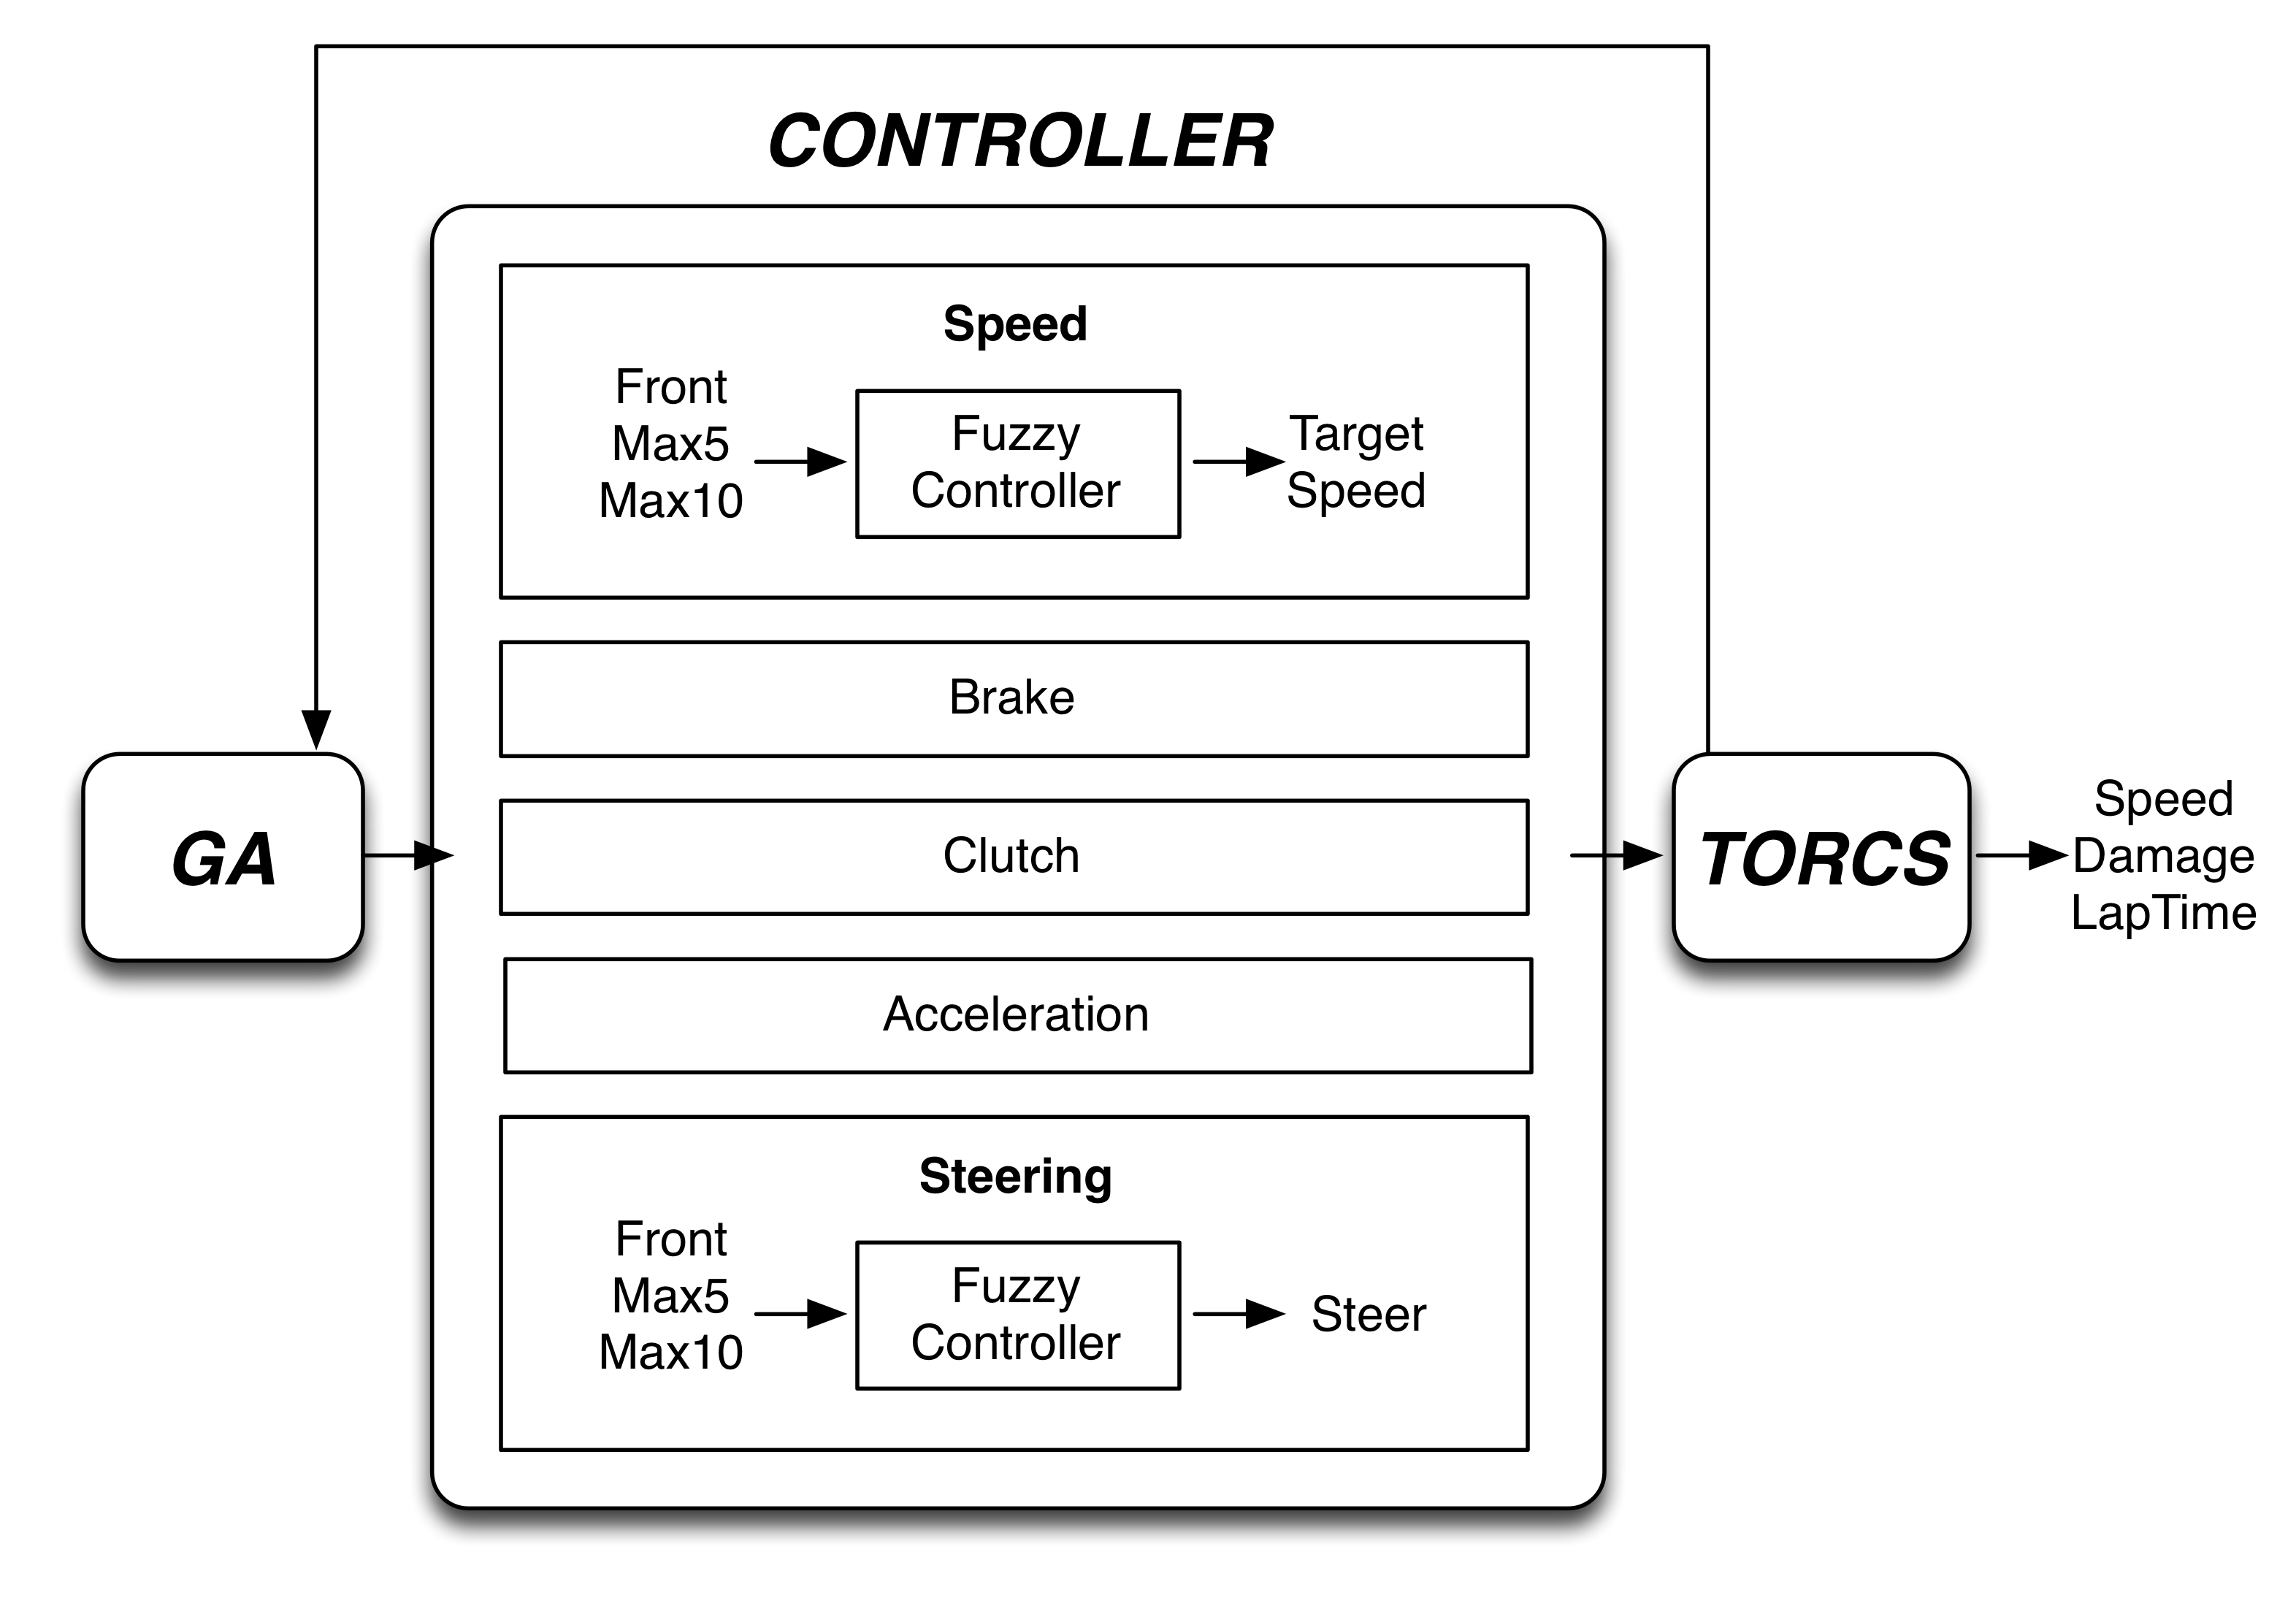
\includegraphics[width=13cm]{fig/flowchart}
	\end{center}
	\caption{Optimization of fuzzy controller flowchart }
% Antonio - Please, explain deeper the figure. It's not easy to understand
 %Mohammed- fixed out
\end{figure}	

%***********************************************
\subsection{Genetic algorithm settings}
%
As previously stated, the designed fuzzy controllers have trapezoidal membership functions given by \ref{eq:trapmf}.
In such a controller, fuzzy rules are applied to linguistic terms. These terms, which qualify a linguistic variable, are defined through membership functions, which, in turn, depend on a set of parameters that `describes' their shape (and operation).
% Antonio - please Mohammed check this text I have added. ;)
 %Mohammed- ok
The parameters to be optimized are  those of all the membership functions that constitute the fuzzy partition of the linguistic variable \cite{ThangG08}.
% Antonio - this sentence seems to be incompleted.
 %Mohammed- fixed out
A trapezoidal membership function in a finite universe of discourse \textit{[a, b]} can be defined by:

\begin{equation}
\mu_{A}(x)= \left \{
\begin{array}{ll}
\frac{x - x_{1}}{x_{2} - x_{1}},& x_{1} \leq x \leq x_{2}\\
1 , &x_{2} \leq x \leq x_{3}\\
\frac{x_{4} - x}{x_{4} - x_{3}},& x_{3} \leq x \leq x_{4}\\
0        ,& else\\	
\end{array}
\right.
\label{eq:trapmf}
\end{equation}
with:
\begin{equation}
x_{1} \leq x_{2} \leq x_{3} \leq x_{4}
\end{equation}
This MF function is defined by four parameters $x_{1}$, $x_{2}$, $x_{3}$ and $x_{4}$ taking their values in the interval \textit{[a, b]} (See Figure \ref{fig:trapeze}).																			
\begin{figure}[!ht] 
	\begin{center}
		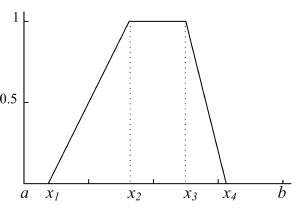
\includegraphics[scale=0.95]{fig/trapese}
		\caption {Trapezoidal MFs}
		\label{fig:trapeze}
	\end{center}
\end{figure}

The input linguistic variables in our problem, \textit{Front, Max5} and \textit{Max10}, are represented by three trapezoidal membership functions (See Table \ref{tab:flouevar}).
More generally, a fuzzy partition with \textit{n} trapezoidal membership functions is defined by \textit{2n} variables (\textit{a =} $ x_{1}$,$x_{2} $,. .., $x_{2n} $ \textit {= b})(Equation \ref{eq:e1}). In this case, the representation is given by the figure \ref{fig:at}
\begin{figure}[!ht] 
	\begin{center}
		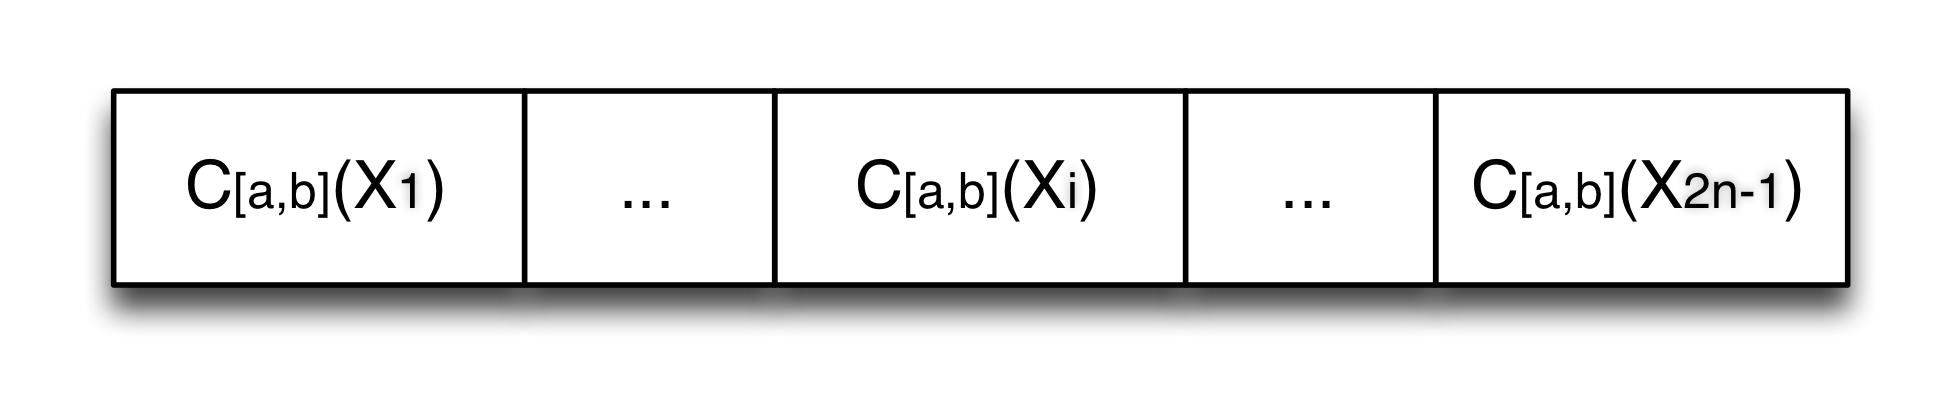
\includegraphics[scale=0.65]{fig/trapezoidal.png}
		\caption {Trapezoidal-shaped MFs coding}
		\label{fig:at}
	\end{center}
\end{figure}
with:
\begin{equation}
a = x_{1} \leq x_{2} \leq...\leq x_{2n-1} \leq x_{2n}=b 	
\end{equation}		

\begin{equation} 
\begin{tabular}{l}
$\mu_{A1}(x)=  \left \{
\begin{array}{ll}
1, &x_{1} \leq x \leq x_{2}\\
\frac{x_{3} - x}{x_{3} - x_{2}}, &x_{2} \leq x \leq x_{3}\\
0        , &x > x_{3}\\
\end{array} 
\right.$		\\ 	
$\mu_{Ai}(x)= \left \{
\begin{array}{ll} 
0, &x \leq x_{2i-2}\\
\frac{x - x_{2i-2}}{x_{2i-1} - x_{2i-2}}, &x_{2i-2} \leq x \leq x_{2i-1},n=2,...,i-1\\
1, & x_{2i-1} \leq x \leq x_{2i}\\
\frac{x_{2i+1} - x}{x_{2i+1} - x_{2i}},& x_{2i} \leq x \leq x_{2i+1}\\
0  , &x > x_{2i+1}\\
\end{array}  
\right.	$		\\
$\mu_{An}(x)= \left \{
\begin{array}{ll} 
0, &x \leq x_{2n-2}\\
\frac{x - x_{2n-2}}{x_{2n-1} - x_{2n-2}},& x_{2n-2} \leq x \leq x_{2n-1}\\
1 ,& x > x_{2n-1} 
\end{array} 
\right.$\\
\label{eq:e1}
\end{tabular}
\end{equation}
	
As we have just seen, a linguistic variable is represented by a number of parameters that depend both on the number and type of used membership functions  \cite{ThangG08}. Also the choice of coding to use for these different parameters depends both on the desired precision on the values and on their range of values.

When the number of parameters is reduced and their ranges of variations are well defined, a GA with a binary coding is largely sufficient to find their optimal values. On the other hand, if the number of parameters becomes important, and their variation interval is not well known, the real coding is the most appropriate \cite{elsayed13}. 
Since our work requires some precision and the variation interval of each parameter is not well known, we have considered a real coding implementation.

The chromosomes of the first population are initialized with random values inside a range of variation \cite{GAs_Goldberg89}, in order to start from feasible values \cite{evo17_blind}. 
% Antonio - another citation is missing.
 %Mohammed- fixed out
The figure \ref {fig:cromosome} illustrates the structure of the chromosome.
%with  :
%% Antonio - Is something missing here? 
%\begin{itemize}
%	\item []$0 = x_{11} \leq x_{12} \leq x_{13} \leq x_{14} \leq x_{15} \leq x_{16} = 100$
%	\item []$0 = x_{21} \leq x_{22} \leq x_{23} \leq x_{24} \leq x_{25} \leq x_{26} = 100$
%	\item []$0 = x_{31} \leq x_{32} \leq x_{33} \leq x_{34} \leq x_{35} \leq x_{36} = 100$
%\end{itemize}
\begin{figure}[!ht]	
	\begin{center}
		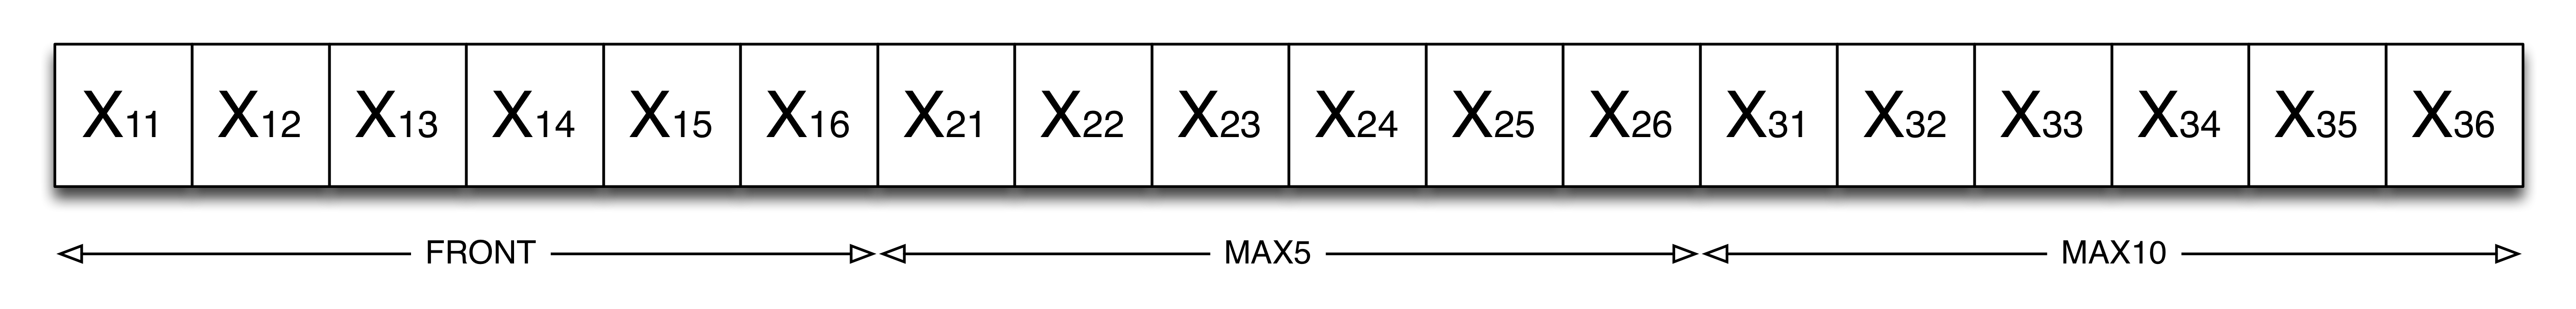
\includegraphics[width=13cm]{fig/chromosome2.png}
		\caption{Chromosome description}
		\label{fig:cromosome}	
	\end{center}	
\end{figure}

Tournament based selection has been used to select chromosomes as parents for genetic operators, while simple arithmetic two point crossover is chosen with non uniform mutation \cite{GAs_Goldberg89}.
% Antonio - we should include a reference to any operator. Moreover, it would be great if we can justify why these operators have been selected (instead of others).

%***********************************************
\subsection{Fitness definition}

The fitness function for optimizing the structure of a fuzzy controller is highly dependent on the application in which the controller is involved. It is therefore not possible to give a general formulation of this function able to adapt to all the peculiarities of a problem. However, we can specify some rules to choose the best evaluation function \cite{elsayed13}.

The fuzzy controller should aim to: 
\begin{itemize}
	\item  Minimize the damage of the car $damage$.
	\item  Minimize the overall race time $RaceTime$.
	\item  Maximize the TopSpeed $MaxSpeed$.		
\end{itemize}

From this goals, we can derive two possible fitness functions:

\begin{description}
	\item[fitness 1:]  
	\begin{equation} \label{fit1}
	\begin{array}{lllll}
	%f_{cout} =  $min$ & \alpha & $. damage$ + & $min$ &\beta & $. temps$ 
	f_{1} =  Min & damage + &\alpha  Min & RaceTime 
	\end{array}
	\end{equation}
	\item[fitness 2:] 
	\begin{equation} \label{fit2}
	\begin{array}{llllll}
	%f_{cout}= min &\alpha & $. dammage$ + & min &\beta & $. temps$ + & min &\gamma & .\frac{1}{vitesse}
	f_{2}= Min & damage + &\alpha Min & RaceTime+ & Min & \beta \frac{1}{MaxSpeed}
	\end{array}
	\end{equation}	
\end{description}

Being $\alpha$ and $\beta$ two weighting parameters to prioritize the importance of the different objectives.
To evaluate the candidate controllers during the evolutionary process, we will make each of them compete in a 20 laps race in E-Track5 circuit 
% Antonio - which kind of race? which track, which conditions, which rivals?
%           This is very important to be mentioned and explained (why have these %           features been selected to correctly evaluate a controller). ;)
and collect the obtained output values ($damage$, $RaceTime$ and $MaxSpeed$) to compute the fitness.


  		
%%%%%%%%%%%%%%%%%%%%%%%%%%%%  SIMULATION RESULTS  %%%%%%%%%%%%%%%%%%%%%%%%%%%%
	
\section{Simulation Results}
	\label{sec:results}
	
This section is dedicated to the performance evaluation of our fuzzy-genetic controller, called \textit{FGC }.
	We first, describe the methodology we have used and next, we present the experimental results of the optimization of the fuzzy-genetic driver and using special criteria in each case.
	
	\subsection{Simulation settings}
	
	TORCS provides several tracks and cars to choose between. In our case, we chose the E-Track5 circuit for its multiple turns and the \textit{car1-tbr1} car of SCR 1 Server\cite{evo17}.\\
	% 
	We have evaluated the fuzzy-genetic controller with the two proposed fitness functions, in order to see which one is appropriate to give the best performances. Thus, we have considered the following bots in the experiments:
	
\begin{enumerate}
\item [- GFC1:] GA-Fuzzy controller with fitness 1 \ref{fit1},
	\item[- GFC2:] GA-Fuzzy controller with fitness 2 \ref{fit2},
	\item AD: Fuzzy controller \cite{evo17} .
\end{enumerate}	
%
Genetic algorithms are used to optimize the parameters of the fuzzy controller developed in \cite{evo17} with the parameters in Table \ref{tab:parametre}:
	
	%%%%%%%%%%%%%%%%%%%%%%%%%%%%%%%%%%%%%%%%%%%%%%%%%%%%%%%%%%%%%%%%%%%%

	\begin{table}[!ht]	
		\centering
		\caption{GA parameters}
		\label{tab:parametre}
		\begin{tabular}{|p{3.6cm}|p{3cm}|}
			\hline \textbf{Population size} & 20 \\
			\hline \textbf{Generations} & 50   \\
			\hline \textbf{Crossover rate$\textit{P}_{\textit{c}}$} &  0.7 \\
			\hline \textbf{Mutation rate $\textit{P}_{\textit{m}}$} &  0.3   \\ 		
			\hline          
		\end{tabular}	
              \end{table}

% All this should have to be eliminated. Either you show the average evolution for several experiments. You also _have_ to do several experiments - JJ              
The evolution of Fitness $f_2$ are presented in Figure  \ref{fig:fit2}, where we could see how the GA converges to the optimal solution along the generations.
\begin{figure}[!h]	
	\begin{center}
		\label{fig:fit2}
		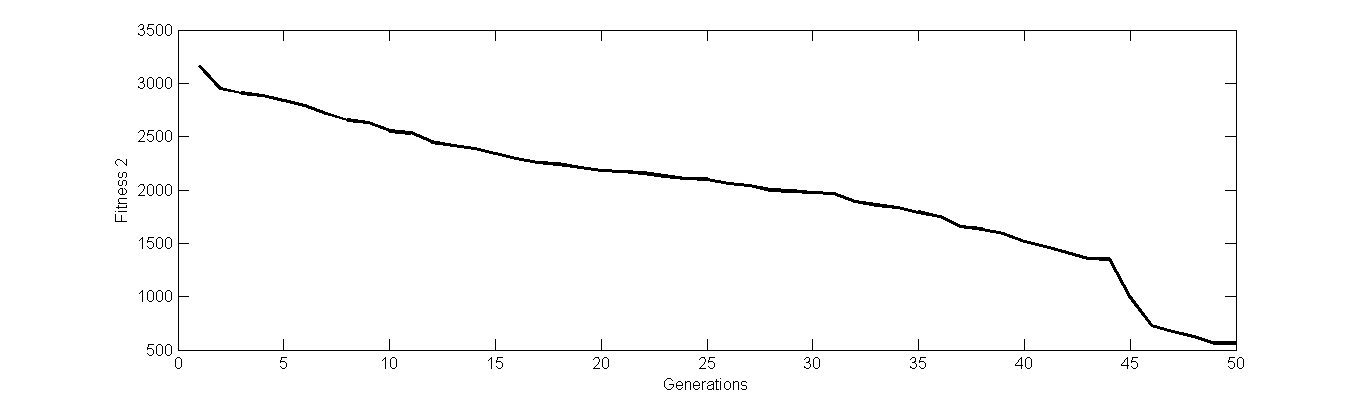
\includegraphics[width=15cm,height=4cm]{fig/fit2}
		\caption{Fitness 2 evolution for 50 generations}	
	\end{center}	
      \end{figure}
      
      After the genetic algorithm ended obtaining the optimal solution, we represented the resulted membership functions in Figures \ref{fig:mffront}, \ref{fig:mfmax5} and \ref{fig:MFMAX10}.
      % These should be examples of results. You can't publish results with a single experiment - JJ


\begin{figure}%
	\centering
	\subfigure[with Fitness 1]{%
		\label{fig:front1}%
		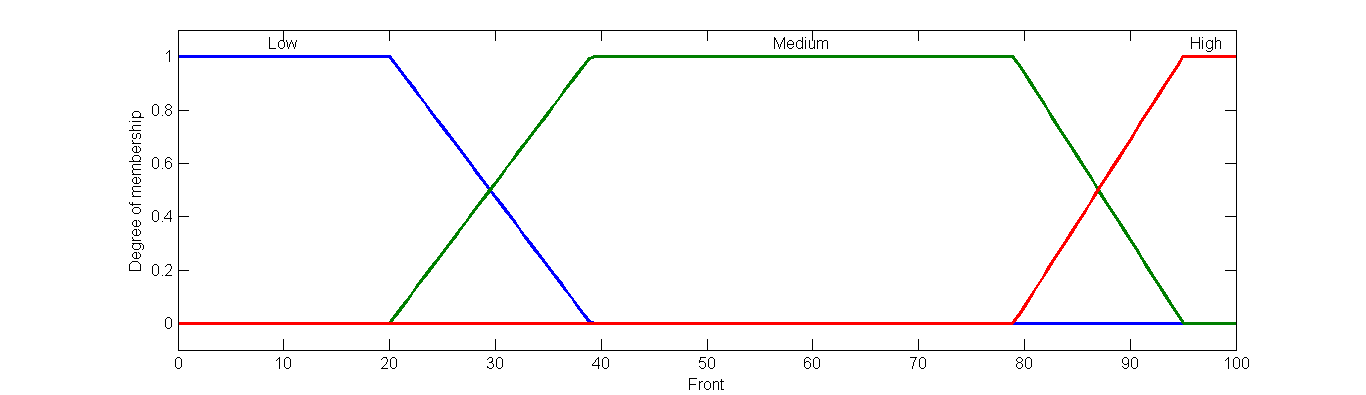
\includegraphics[width=0.6\textwidth,height=3cm]{fig/MFFRONT}}%
	\subfigure[with Fitness 2]{%
		\label{fig:front2}%
		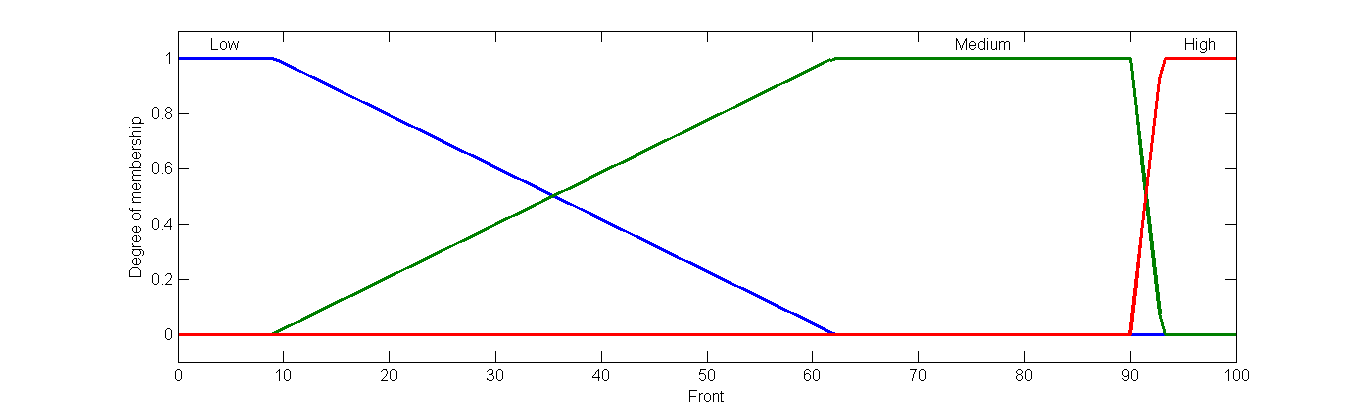
\includegraphics[width=0.6\textwidth,height=3cm]{fig/MFFRONT2}}%
	\caption{Front input MFs with GA}
	\label{fig:mffront}
\end{figure}

\begin{figure}%
	\centering
	\subfigure[with Fitness 1]{%
		\label{fig:fmax51}%
		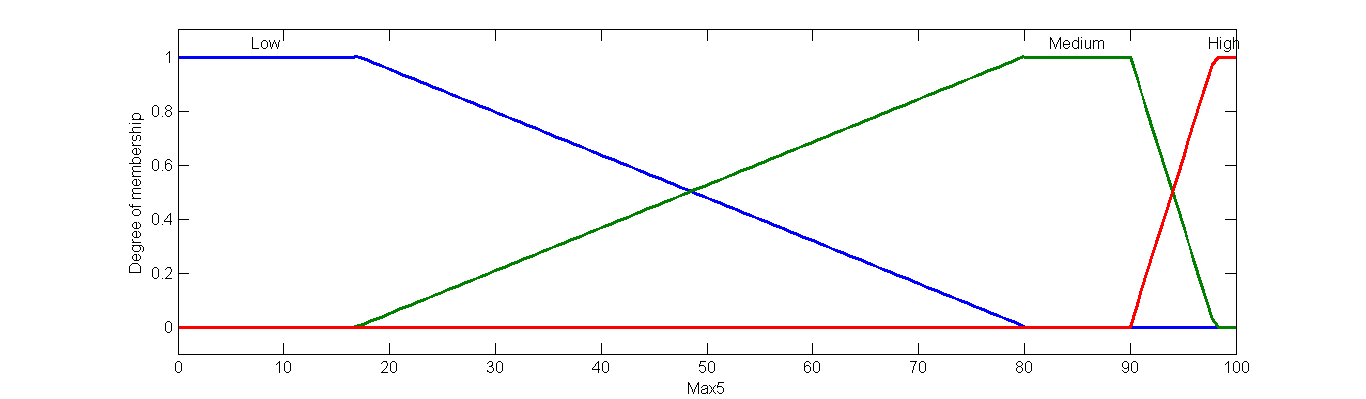
\includegraphics[width=0.6\textwidth,height=3cm]{fig/MFFMAX5}}%
	\subfigure[with Fitness 2]{%
		\label{fig:Fmax52}%
		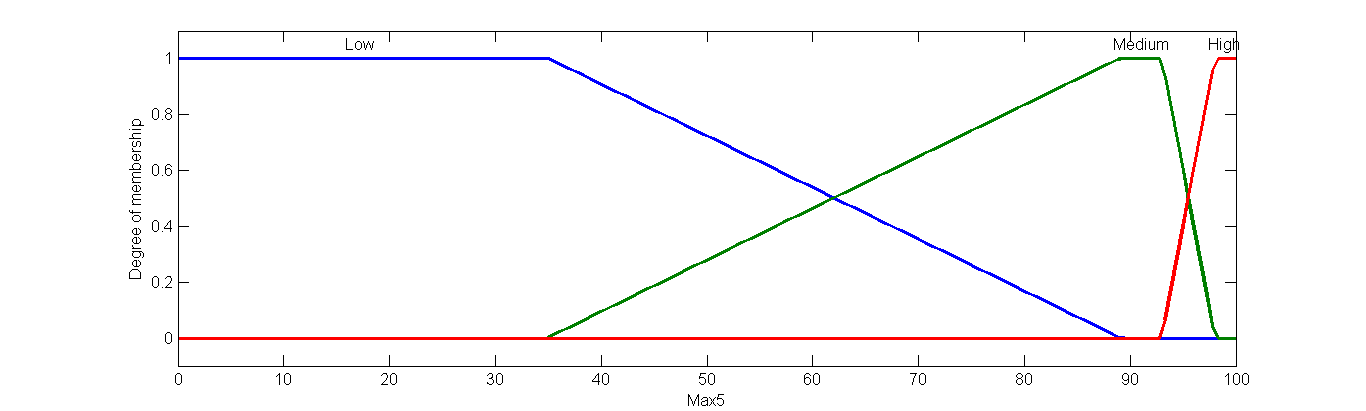
\includegraphics[width=0.6\textwidth,height=3cm]{fig/MFFMAX52}}%
	\caption{Max5 input MFs with GA}
	\label{fig:mfmax5}%
\end{figure}

\begin{figure}%
	\centering
	\subfigure[with Fitness 1]{%
		\label{fig:MFMAX101}%
		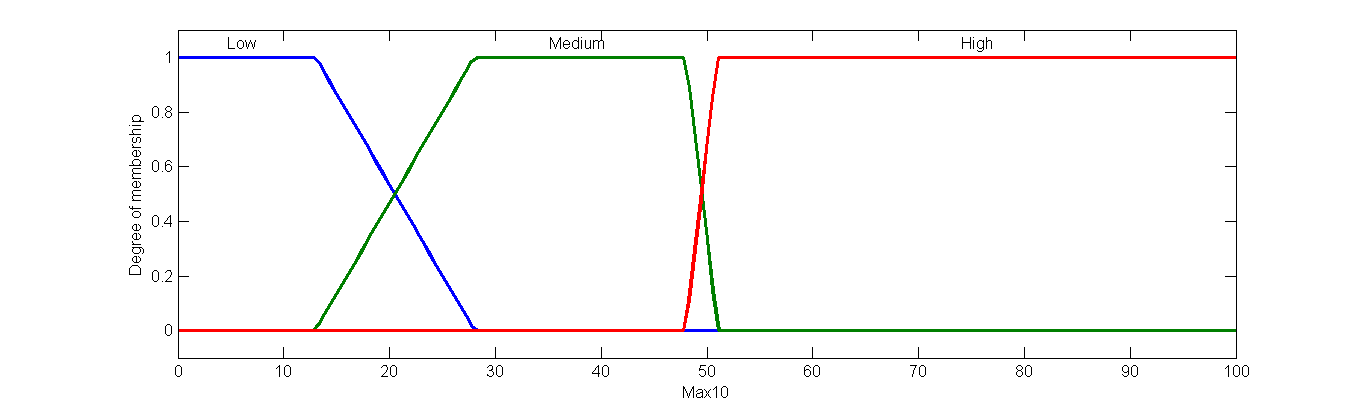
\includegraphics[width=0.6\textwidth,height=3cm]{fig/MFMAX10}}%
	\subfigure[with Fitness 2]{%
		\label{fig:MFMAX102}%
		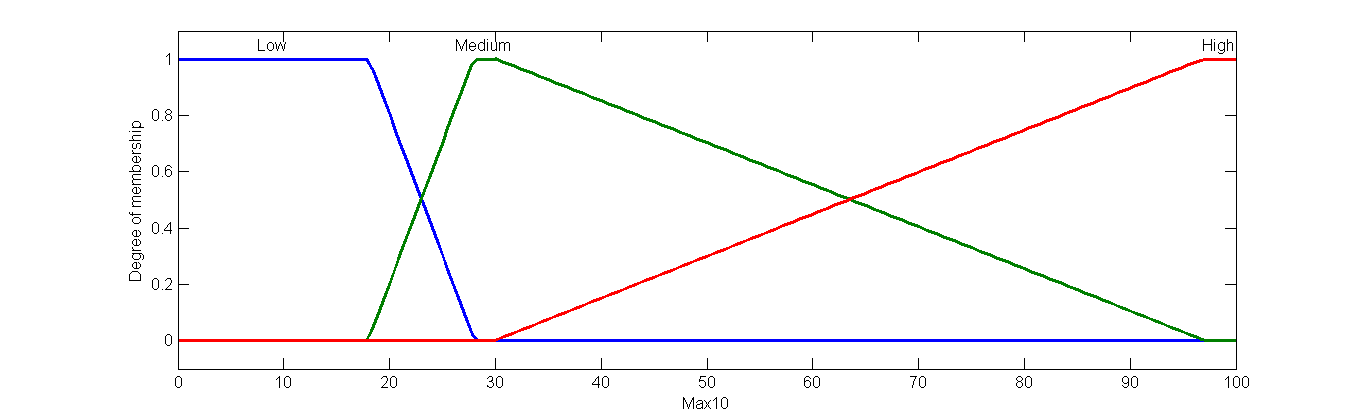
\includegraphics[width=0.6\textwidth,height=3cm]{fig/MFMAX102}}%
	\caption{Max10 input MFs with GA}
		\label{fig:MFMAX10}%
\end{figure}



%%%%%
\subsection{GA-Fuzzy  controller in practice race} 
The genetic based fuzzy controllers obtained from the last section are tested in practice race where the two controllers $GFC1$ and $GFC2$ and $AD$ (fuzzy controller) will run each one for 20 laps in E-Track 5 which we used in the evolution approach and tested in E-Road track. The results are in Table \ref{resultat20}.
\begin{table}[!ht]
	\centering
	\caption{Results of the three controllers in a 20 laps practice race}
	\label{resultat20}
	\begin{tabular}{|c|p{2.75 cm}|p{2.75cm}|p{2.75cm}}
		\hline
		\multicolumn{4}{|c|}{{\large \textbf{E-Track 5}}}  \\ \hline
		\hline \textbf{20 laps} & \textbf{AD} & \textbf{GFC1} & \textbf{GFC2}  \\
		\hline Best Lap Time         & 29:70 & 30:03 & 29:50 \\
		\hline TopSpeed          & 209 & 216 & 216\\
		\hline MinSpeed          & 168 & 148 & 182 \\
		\hline Lastlap Time       & 29:79 &  30:03 & 29:50\\
		\hline Damages          & 936 & 0 & 0\\
		\hline
		\multicolumn{4}{|c|}{{\large \textbf{E-Road}}}  \\ \hline
		\hline \textbf{20 laps} & \textbf{AD} & \textbf{GFC1} & \textbf{GFC2}  \\
		\hline Best lap Time         & 02:31:71    & 02:26:72       & 02:26:54  \\
		\hline TopSpeed          & 206         & 205            &  208 \\
		\hline MinSpeed          & 30          & 39             & 37  \\
		\hline Lastlap Time       & 03:12:79    &  02:42:26      &  02:33:36 \\
		\hline Damages          &   0         & 0              & 0  \\
		\hline 
	\end{tabular}
\end{table}
From the table, we can see that the fuzzy controllers optimized by genetic algorithms have given the best results minimizing the global race time and damages ($0$ in  the two GA based fuzzy controllers ) while the AD controller has finished the practice race with some damages.
We notice also that the GFC controller has run with a higher top speed then GFC1. This is due to to the inclusion of Topspeed in the fitness confirming that GFC2 is the best controller.

\subsection{GA-Fuzzy controllers in a real race}
The considered fuzzy controllers have been used in real race with five controllers from each team integrated with TORCS. The Table \ref{tab:adreal}, \ref{tab:gfc1real}, \ref{tab:gfc2real} illustrate the results obtained in a five laps real race. We note that the obtained ranking by the controllers $GFC1$,   $GFC2$ was third and second respectively. 
While  the point of view of race time, GFC2 has a better time than GFC1. For the damage, GFC1 and GFC2 finished the race without recording any damage On the other hand, the AD controller was not able to avoid high damages in the track.


\begin{table}[!ht]
	\caption{Results of GFC1 in a real race}
	\label{tab:gfc1real}
	\begin{tabular}{|p{2.3cm}|p{1.75 cm}|p{1.75 cm}|p{1.75 cm}|p{1.75 cm}|p{1.75 cm}|p{1.75 cm}|}
		\hline \textbf{E-track5} &   \textbf{GFC1} & \textbf{berwin 10} & \textbf{bt 3} &\textbf{damned 2} & \textbf{inferno 5} & \textbf{tita 10}  \\
		\hline \textbf{Ranking} & 3/6&4/6&1/6&5/6&2/6&6/6\\			
		\hline \textbf{Race Time}	& 02:30:74\newline+35:70&02:30:74\newline+1lap&02:30:74&02:30:74\newline+1lap&02:30:74\newline+12:13&02:30:74\newline+1lap\\	
		\hline \textbf{Best Lap}&35:65& 36:39&28:57&36:83&30:53&35:39\\	
		\hline \textbf{Maxspeed}& 196&202&231&192&226&202\\	
		\hline \textbf{Damages}& 0&0&0&603&0&471 \\	
		\hline 
	\end{tabular}
\end{table}
\begin{table}[!ht]
	\caption{Results of GFC2 in a real race }
	\label{tab:gfc2real}
	\begin{tabular}{|p{2.3cm}|p{1.75 cm}|p{1.75 cm}|p{1.75 cm}|p{1.75 cm}|p{1.75 cm}|p{1.75 cm}|}
		\hline \textbf{E-track5} & \textbf{GFC2}&\textbf{berwin 10} & \textbf{bt 3} &\textbf{damned 2} & \textbf{inferno 5} & \textbf{tita 10}  \\
		\hline \textbf{Ranking} & 2/6&4/6&1/6&6/6&3/6&5/6\\			
		\hline \textbf{Race Time}	& 02:30:83\newline +03:99&  02:30:83\newline+1lap&02:30:83&02:30:83\newline+1lap&02:30:83\newline+08:35&02:30:83\newline+1lap\\	
		\hline \textbf{Best Time}& 29:82 &36:38&28:35&37:04&30:53&36:00\\	
		\hline \textbf{Maxspeed}& 214&202&230&188&226&204\\	
		\hline \textbf{Damages}& 0& 0 & 343&1230&0&668\\	
		\hline 
	\end{tabular}
\end{table}
\begin{table}[!ht]
	\caption{Results of AD in a real race}
	\label{tab:adreal}
	\begin{tabular}{|p{2.3 cm}|p{1.75 cm}|p{1.75 cm}|p{1.75 cm}|p{1.75 cm}|p{1.75 cm}|p{1.75 cm}|}
		\hline \textbf{E-track5} & \textbf{AD} & \textbf{berwin 10} & \textbf{bt 3} &\textbf{damned 2} & \textbf{inferno 5} & \textbf{tita 10}  \\
		\hline \textbf{Ranking} & 6/6&5/6&1/6&4/6&2/6&3/6\\			
		\hline \textbf{Race Time}	& 02:31:83\newline+5laps&02:31:83\newline+1lap&02:31:83&02:31:83\newline+1lap&02:31:83\newline+21:32&02:31:83\newline+33:43 \\	
		\hline \textbf{Best Time}& 00:00&37:25&28:60&36:28&31:47&35:84\\	
		\hline \textbf{Maxspeed}& 111&202&230&189&225&202\\	
		\hline \textbf{Damages}& 10786&465&5&0&2394&0 \\	
		\hline 
	\end{tabular}
\end{table}



	\section{Conclusions and Future Work} 
\label{sec:conclusions}

In this work, we presented a genetic approach to optimize and improve an existing fuzzy driver for TORCS simulator, which combines two sub-controllers, one to calculate the target speed and the other for the direction (steer).
In the evolution approach, we tested two fitness functions, one with the Best Time, the car damage and the other one consider also the top speed.
The fuzzy-genetic controllers thus obtained were compared with the original AD controller and whose parameters are determined empirically, the comparison was made first without opponents and then, with cars from the TORCS teams.
The obtained results are interesting in the context where the designed controllers were ranked among the first ones in the evaluation races, with the minimum of damage.

Nevertheless, these results can be improved by extending the evaluation of population controllers in the Genetic algorithm to other tracks and not just one to allow the elected controller to practice effectively in multiple tracks and in real-life situations.
In other hand, we can also try to optimize and tune automatically the rule base of the fuzzy controller.


\section*{Acknowledgments}

% This work has been supported in part by: Ministerio espa\~{n}ol de
% Econom\'{\i}a y Competitividad under project TIN2014-56494-C4-3-P
% (UGR-EPHEMECH).
Hidden for double blind\\
Taking this much space.

	\bibliographystyle{splncs03}
	\bibliography{fuzzy_torcs}
	
	
	
	
	
	
\end{document}
